%! Author = Raffaele
%! Date = 17/01/2024

\newpage
\section{Il gioco}\label{sec:gioco}

\begin{figure}
    \centering
    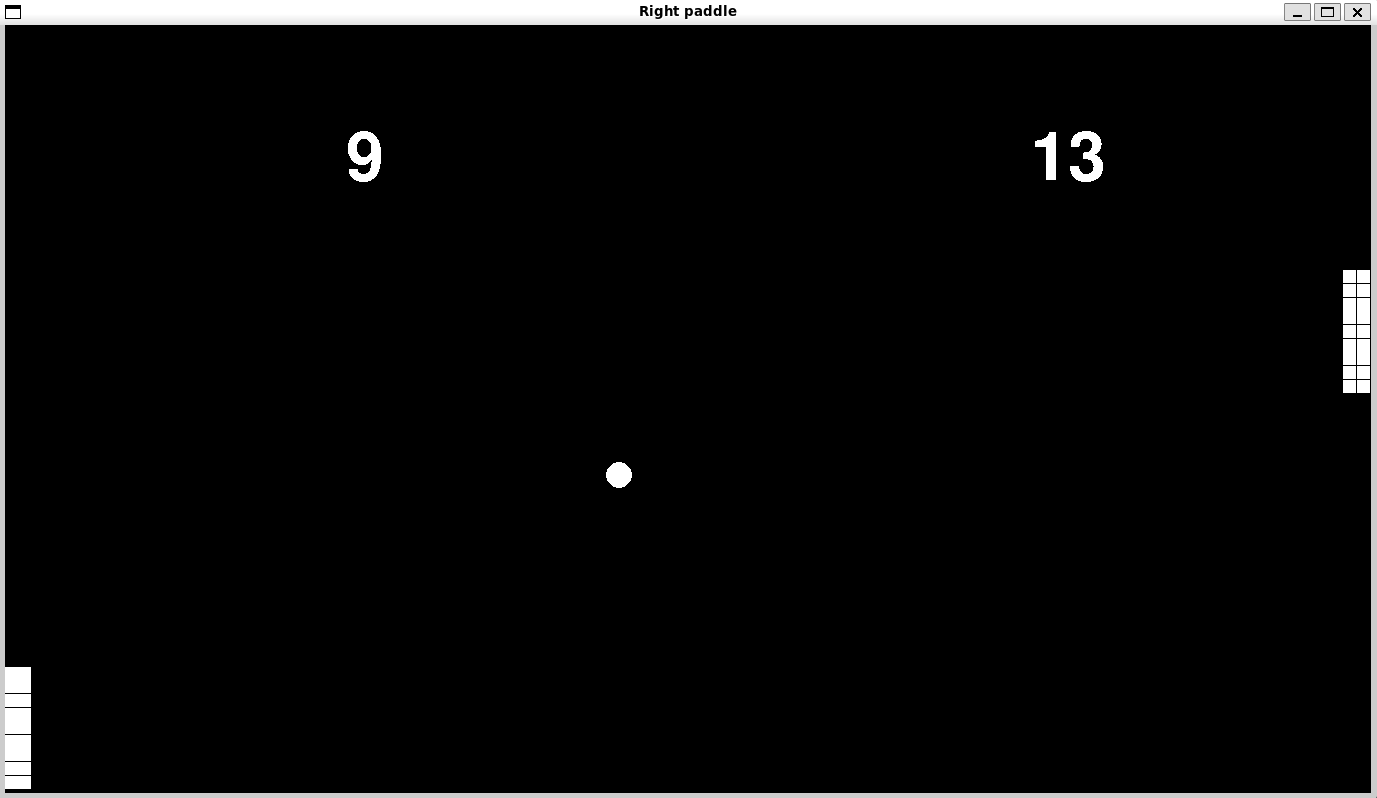
\includegraphics[scale=0.4]{img/gioco}
    \caption{Immagine dell'interfaccia di gioco}
    \label{fig:gioco}
\end{figure}

Il gioco viene avviato tramite linea di comando passando opzionalmente l'indirizzo dell'altro peer
(se questi non viene inserito, l'applicazione utilizza l'indirizzo di loopback). \\
Dopo aver passato gli argomenti ottenuti da linea di comando, il programma richiama la funzione \textit{peer\_run}
che è divisa in due parti:
\begin{itemize}
    \item \textbf{Creazione del peer e delle variabili di gioco} (Figura \ref{fig:inizializzazione})
    Vengono inizializzate tutte le variabili necessarie al funzionamento della partita, tra cui la griglia di gioco,
    la classe del peer locale e le variabili necessarie al funzionamento di \textit{pygame}
    \item \textbf{Il game loop} (Figura \ref{fig:game-loop}), ovvero il loop del gioco vero e proprio, composto come segue:
    \begin{itemize}
        \item Ottenimento dell'input da parte dell'utente, il tasto W muove la racchetta verso l'alto, mentre il
        tasto S la muove verso il basso.
        \item Invio del pacchetto UDP contenente le informazioni sulla propria racchetta e ricezione del pacchetto
        della controparte.
        \item A questo punto, il seeder gestisce opportunamente il movimento della pallina, se la pallina esce
        da un lato della griglia, procede ad aggiornare opportunamente lo scorekeeper, e invia i dati alla controparte. \\
        Nel mentre l'altro peer si limita ad ottenere i dati dalla controparte.
        \item Infine, entrambi i peer aggiornano la propria griglia in base ai dati posseduti e aggiornano il display.
    \end{itemize}
\end{itemize}

\begin{figure}
    \begin{verbatim}
        # Import omessi per semplicità

        def peer_run(args):
            # inizializzazione delle variabili
            grid = Grid()
            pygame.init()
            pygame.font.init()
            screen = pygame.display.set_mode((SCREEN_WIDTH, SCREEN_HEIGHT))
            clock = pygame.time.Clock()

            # creazione del peeer
            peer = Peer(args.peer_id)
            peer.set_other_peer(args.other_peer_address)

            # LEFT_PADDLE_ID è 0
            if peer.id == LEFT_PADDLE_ID:
                pygame.display.set_caption("Left paddle")
            else:
                pygame.display.set_caption("Right paddle")

            # continua...
    \end{verbatim}
    \caption{Inizializzazione del gioco}
    \label{fig:inizializzazione}
\end{figure}

\begin{figure}
    \begin{verbatim}
        # main game loop
        # alcune parti omesse per semplicità
        while True:
            # gestione dell'input
                # se viene premuto W...
                peer.controlled_paddle.velocity = -1
                # se viene premuto S...
                peer.controlled_paddle.velocity = 1

            # scambio dei dati delle proprie racchette
            peer.controlled_paddle.move()
            peer.send_data(peer.controlled_paddle)
            peer.receive_and_replace_object_data()

            if peer.ball.seeder_id == peer.id:
                # la pallina viene mossa oportunamente
                # e la posizione aggiornata viene inviata
                peer.send_data(peer.ball)
                if peer.ball.is_out():
                    if peer.ball.pos_x <= 0:
                        peer.scorekeeper.add_score(left_paddle_scored=False)
                    elif peer.ball.pos_x >= GRID_WIDTH:
                        peer.scorekeeper.add_score(left_paddle_scored=True)
                    peer.ball.reset_position()
                    peer.ball.set_random_velocity()
                    peer.send_data(peer.ball)
                    peer.send_data(peer.scorekeeper)
            # l'altro peer ottiene semplicemente i dati
            else:
                peer.receive_and_replace_object_data()
                peer.receive_and_replace_object_data()

            # aggiornamento della griglia,
            # del codice è stato omesso per semplicità
            grid.update_grid(  # args  )
            grid.display(screen)
            peer.scorekeeper.display(screen)
            pygame.display.flip()
            clock.tick(FPS)
    \end{verbatim}
    \caption{Il game loop}
    \label{fig:game-loop}
\end{figure}
